% !TeX spellcheck = en_US
\documentclass[aspectratio=1610]{beamer}
\mode<presentation>
{
  \usetheme{Boadilla}
  \setbeamercovered{transparent}
  
  \definecolor{cobalt}{rgb}{0.0, 0.02 0.50}
  
  \usecolortheme[named=cobalt]{structure}
  %\usecolortheme{lily}
  %\setbeamercolor{headline}{fg=cyan!80!black}
  % \setbeamercolor{frametitle}{bg=white}.
}

\makeatletter
\define@key{beamerframe}{wide}[10pt]{%
	\def\beamer@cramped{\itemsep #1\topsep0.5pt\relax}}
\makeatother
	

\usepackage[english]{babel}
\usepackage[utf8]{inputenc}
\usepackage{times}
\usepackage[T1]{fontenc}
\usepackage{array}
\usepackage{xcolor}
\usepackage{colortbl}
\usepackage{booktabs}

\title[Fall - Lecture 6] % (optional, use only with long paper titles)
{Macroeconomic Theory and Policy: Lecture  6 (Ch. 5)}

\author[University of Toronto] % (optional, use only with lots of authors)
{}
\date[] % (optional, should be abbreviation of conference name)

\begin{document}

\begin{frame}
  \titlepage
\end{frame}

\begin{frame}[wide]{What are You Going to Learn (Ch. 5)}
	\begin{itemize}
		\item Solow Growth Model
		\item How capital accumulates over time
		\item How diminishing marginal product of capital explains differences in growth rates across countries
		\item The principle of transition dynamics
		\item The limitations of capital accumulation, although a significant part of economic growth is still left unexplained
	\end{itemize}
\end{frame}

\begin{frame}[wide]{Solow Growth Model}
	\begin{itemize}
		\item The Solow growth model builds on the production model
		\begin{itemize}
			\item It provides us with a starting point to discuss why growth differs across countries
			\item The model has been extended in a number of important directions
			\item Foundation for modern economic growth theory (and a lot of empirical work)
		\end{itemize}		
	\end{itemize}
\end{frame}

\begin{frame}[wide]{Solow Growth Model}
	\begin{itemize}
		\item There are a few key differences:
		\begin{itemize}
			\item Capital is endogenized: converted from an exogenous to an endogenous variable
			\item Augments the production model with capital accumulation
			\begin{itemize}
				\item Agents in the model can accumulate tools, machines, computers, and buildings over time
			\end{itemize}
			\item The accumulation of capital is a possible engine of long-run economic growth
			\item In other words, some countries are richer than others because they invest more in accumulating capital
		\end{itemize}
		
	\end{itemize}
\end{frame}

\begin{frame}[wide]{Setting Up the Model: Production Function}
	\begin{itemize}
		\item Add an equation for the accumulation of capital over time to the production model
		\item The Cobb-Douglas production function:
		\begin{itemize}
			\item Constant returns to scale
			\item Increasing in both capital and labor
		\end{itemize}
		\item Variables are time subscripted ($t$)
		\[Y_t = F(K_t,L_t) = \bar{A} K_t^{\alpha} L_t^{1-\alpha}\]
		The $Y_t$ is now the output in period $t$, $K_t$ is the capital in period $t$ and $L_t$ is the labour used in period $t$
	\end{itemize}
\end{frame}

\begin{frame}[wide]{Setting Up the Model: Resource Constraint}
	\begin{itemize}
		\item Output can be used for consumption or investment
		\[Y_t = C_t + I_t\]
		$C_t$ is the consumption in period $t$, $I_t$ is the investment in period $t$
		\item Assumes no imports or exports (i.e., closed economy)
	\end{itemize}
\end{frame}

\begin{frame}[wide]{Setting Up the Model: Capital Accumulation}
	\begin{itemize}
		\item Goods invested for the future determine the accumulation of capital
		\item Capital accumulation equation:
		\[K_{t+1} = K_t + I_t - \delta K_t\]
		\begin{itemize}
			\item [] $K_{t+1}$ is the next year's capital
			\item [] $K_{t}$ is the this year's capital
			\item [] $I_t$ is this year's investment
			\item [] $\delta K_t$ is the depreciation of capital
			\item [] $\delta$ is the depreciation rate which usually assume to be $0<\delta <1$
		\end{itemize}
		\item We will use $\bar{d}$ and $\delta$ interchangeably. Typically, the estimate is around 7 to 10\% annually
	\end{itemize}
\end{frame}

\begin{frame}[wide]{Setting Up the Model: Capital Accumulation}
	\begin{itemize}
		\item Change in capital stock defined as
		\[\Delta K_{t+1} =K_{t+1} -K_t \]
		then,
		\[\Delta K_{t+1} = I_t - \delta K_t\]
		Future capital depends on investment today
		\item Today’s capital is a result of investments in the past
		\begin{itemize}
			\item This applies for all time periods in the model other than the first
			\item So, we assume the economy is endowed with some initial level of capital at $t = 0$
		\end{itemize}
	\end{itemize}
\end{frame}

\begin{frame}[wide]{Setting Up the Model: Labour}
	\begin{itemize}
		\item For simplicity, labor supply is assumed to be inelastic and is given endogenously
		\[L=\bar{L}\]
		\item A simple extension would be allowing for population growth, which we will cover later
	\end{itemize}
\end{frame}	

\begin{frame}[wide]{Setting Up the Model: Investment}
	\begin{itemize}
		\item The economy consumes a fraction of output and invests the rest
			\[I_t = \bar{s}Y_t\]
		where $\bar{s}$ is the fraction of output invested ($0<\bar{s}<1$)
		\vspace{4mm}
		\item This implies
		\[C_t = (1-\bar{s})Y_t\]
		Consumption is the share of output not invested
		\item We will go through a model of investment and consumption later in the term
	\end{itemize}
\end{frame}

\begin{frame}[wide]{Five Equations and Five Unknowns}
	\begin{itemize}
		\item Endogenous variables: $Y_t,K_t,L_t,I_t,C_t$
		\item Parameters: $\bar{A}, \bar{s}, \delta, \bar{L}, \bar{K}_0$
		\item Five equations:
			\[Y_t=\bar{A}K_t^{\alpha}L_t^{1-\alpha}\]
			\[\Delta K_{t+1} = I_t - \delta K_t\]
			\[L_t = \bar{L}\]
			\[Y_t = C_t + I_t\]
			\[I_t = \bar{s} Y_t\]
		\item This is a  dynamic model in which each equation holds at each point in time
	\end{itemize}
\end{frame}

\begin{frame}[wide]{Some more Differences between Solow and Production Model}
	\begin{itemize}
		\item In the Solow model, we have added dynamics in the form of capital accumulation
		\vspace{3mm}
		\item The Solow model leaves out the markets for capital and labor and the corresponding prices—the rental price of capital ($r$) and the wage rate ($w$)
		\vspace{1mm}
		\begin{itemize}
			\item This is a simplification that makes the model easier to solve
		\end{itemize}
		\vspace{3mm}
		\item The consumption equation is part of the model, but it would be redundant to include
	\end{itemize}
\end{frame}

\begin{frame}[wide]{Variables: Stock and Flow}
	\begin{itemize}
		\item Stock: A quantity that survives from period to period
		\begin{itemize}
			\item Capital in Solow model is a stock variables
			\begin{itemize}
				\item e.g., Tractor, house, factory
			\end{itemize}
			\item Think of it as the saving you have in the saving amount
		\vspace{3mm}
		\end{itemize}
		\item Flow: A quantity that lasts a single period
		\begin{itemize}
			\item Output, investment consumption are a flow variables
			\item Think of it as the amount you just deposit to the saving account
		\end{itemize}
		\vspace{3mm}
		\item The change in a stock is a flow
		\begin{itemize}
			\item Change in the capital stock equals the flow of investment
		\end{itemize}
	\end{itemize}
\end{frame}

\begin{frame}[wide]{Prices and the Real Interest Rate}
	\begin{itemize}
		\item We can add the wage and rental rate to our model, we would have 
		\begin{itemize}
			\item Two more endogenous variables and two more equations
			\[w = MPL \text{  and  } r = MPK	\]
			\item Omitting them does not change the basic behaviour of the model
		\end{itemize}
	\end{itemize}
\end{frame}

%\begin{frame}[wide]{Prices and the Real Interest Rate}
%	\begin{itemize}
%		\item  However, another important price to consider is the real interest rate
%		\begin{itemize}
%			\item The real interest rate is the amount a person can earn (pay) by saving (borrow) one unit of \textit{output} for a period
%			\item This is a real variable because it is measured in units of output (or constant dollars), rather than in nominal dollars
%		\end{itemize}
%		
%		\item Consider the source of the supply of capital in an economy comes from the decision by households to forgo consumption and save instead
%		\item In a competitive market of capital, 
%		\[\text{Real interest rate} = \text{rental price of capital} = \text{MPK}\]
%		\begin{itemize}
%			\item Capital owner cannot charge a higher rate. Also, they won't charge a lower rate as the owner would lost compare to saving
%		\end{itemize}
%	\end{itemize}
%\end{frame}

\begin{frame}[wide]{Saving in Solow Model}
	\begin{itemize}
		\item National income identity also hold in the Solow model
		\item The saving is just the difference between income and consumption
				\[\text{Saving} = Y_t - C_t = I_t = \text{Investment}\]
		\item Each unit of saving gets used as a unit of investment
		\[\text{Saving} = \text{investment} = \text{supply of capital} \]
	\end{itemize}
\end{frame}

\begin{frame}[wide]{Solving the Solow Model }
	\begin{itemize}
		\item The model needs to be solved at every point in time, which cannot be done algebraically
		\begin{itemize}
			\item There are infinite amount of $t$
		\end{itemize}
		\item Two ways to make progress:
		\begin{itemize}
			\item Show a graphical solution
			\item Solve the model in the long run
		\end{itemize}
		\item Begin by combining equations algebraically
	\end{itemize}
\end{frame}

\begin{frame}[wide]{Solving the Solow Model  }
	\begin{itemize}
		\item Convert $Y$, $K$ and $I$ into per capita term
		\[y_t = Y_t/L_t \text{, } k_t = K_t/L_t \text{ and } i_t = I_t/L_t\]
		\begin{itemize}
			\item Since we assume $L=\bar{L}$, we can solve the model at level as well (see extra question)
		\end{itemize}
		\item Combine the investment allocation ($i_t = \bar{s}y_t$) and capital accumulation equation ($\Delta k_{t+1} = i_t -\delta k_t$)
		\[\Delta k_{t+1} = \bar{s}y_t -\delta k_t\]
		\[\text{Change in Capital per capita} = \text{Net Investment per capita}\]
%		\item Substitute the fixed amount of labor into the production function
%		\[Y_t = \bar{A} K_t^\alpha \bar{L}^{1-\alpha}\]
%		\item Combine the two equations:
%		\[\Delta K_{t+1} = \bar{s}\bar{A}  \bar{L}^{1-\alpha} K_t^\alpha -\delta K_t\]
	\end{itemize}
\end{frame}

\begin{frame}[wide]{The Solow Diagram}
	\begin{itemize}
		\item Investment is $i_t = \bar{s}y_t = \bar{s}\bar{A} k_t^\alpha$
		\begin{itemize}
			\item with the usual assumption that $0<\alpha<1$
			\item increasing with diminishing return
		\end{itemize}
		\item Depreciation is $\delta K_t$, which is linear
		\begin{figure}
			\centering
			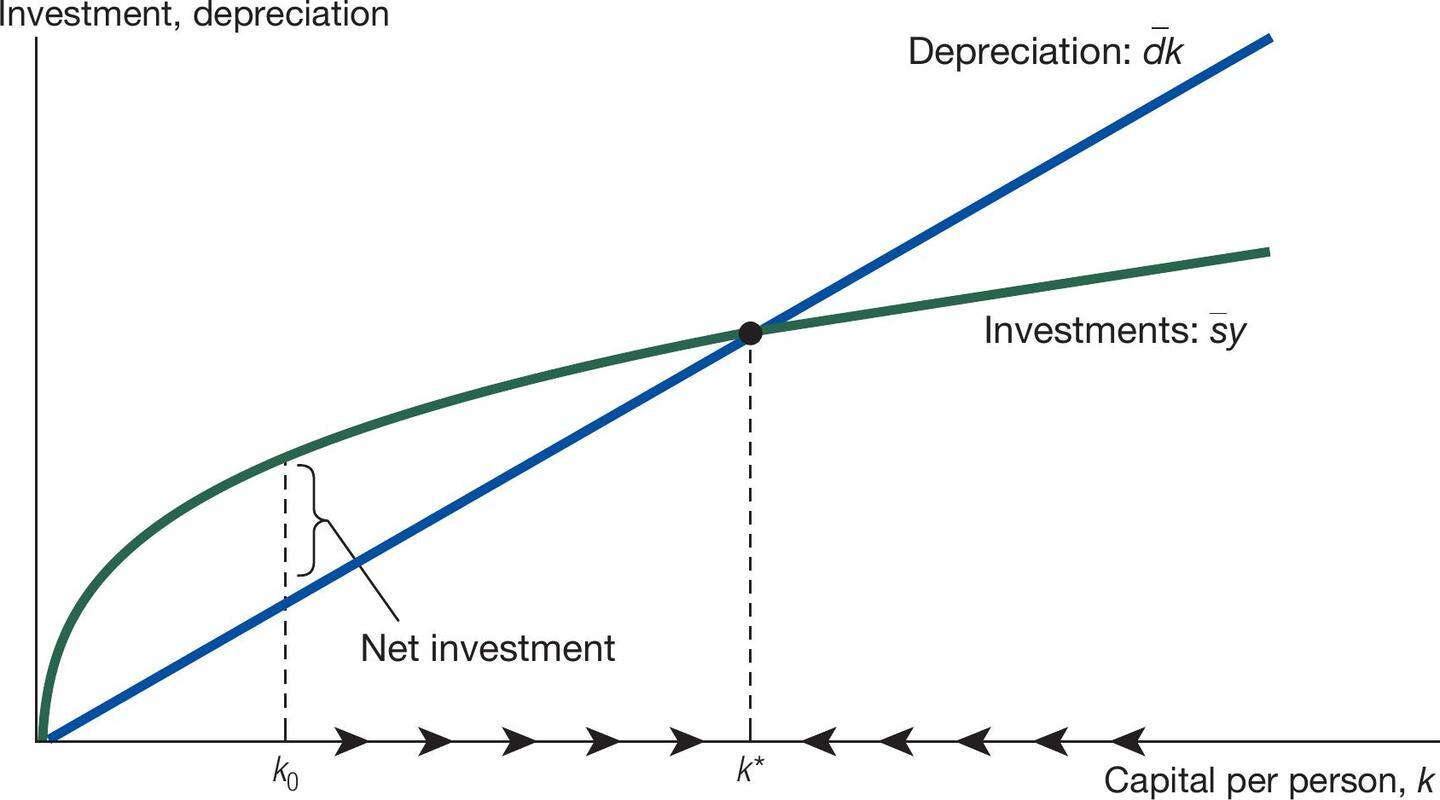
\includegraphics[width=0.7\linewidth]{Figures/MACRO6_FIG05.01}
		\end{figure}
		
	\end{itemize}
\end{frame}

\begin{frame}[wide]{Using the Solow Diagram}
	\begin{itemize}
		\item If the amount of investment > depreciation, $sy_t>\delta k_t$
		\begin{itemize}
			\item Capital stock will increase until the amount of investment being undertaken is equal to the amount of capital that wears out through depreciation $sy_t=\delta k_t$
			\item This is called the steady state, capital stock will stay at this value of capital forever and the change in capital is equal to 0
		\end{itemize} 
		\vspace{4mm}
		\item If depreciation is greater than investment, , $sy_t<\delta k_t$, the economy converges to the same steady state as above
		\begin{itemize}
			\item  Capital stock will increase until the amount of investment being undertaken is equal to the amount of capital that wears out through depreciation
		\end{itemize}
	\end{itemize}
\end{frame}

\begin{frame}[wide]{Model Dynamics}
	\begin{itemize}
		\item When not in the steady state, the economy exhibits a change in capital toward the steady state
		\item As $k$ moves to its steady state, output will also move to its steady state
		\item At the steady state, all endogenous variables are steady
		\item \textit{Transition dynamics} take the economy from any possible initial level of capital to the steady state
		\item No matter what level of initial capital we choose, if we wait long enough, the economy will converge to the steady state, $k^*$
	\end{itemize}
\end{frame}

\begin{frame}[wide]{The Solow Diagram with Output}
	\begin{itemize}
		\item We can also plot the production function to see how output evolves over time
		\item As transition dynamics take the economy from $k_0$ to $k^*$ output rises over time from $y_0$ to $y^*$
		\item Consumption can also be plotted, it  is the difference between output and investment
	\end{itemize}
	\begin{figure}
		\centering
		\includegraphics[width=0.5\linewidth]{"Figures/MACRO6_FIG05.02"}
	\end{figure}
	
\end{frame}

\begin{frame}[wide]{Solving for the Steady State}
	\begin{itemize}
		\item We can solve mathematically for the steady-state level of capital
		\begin{itemize}
			\item Recall that steady state is a long-run equilibrium where, if the model’s variables equal a certain set of values, they will never again change from these values
		\end{itemize}
		\item In the steady state, investment equals depreciation (i.e., $\Delta K =0 $)
		\[ \Delta k = 0 = \bar{s}y^* -\delta k^* \implies \bar{s}y^* =\delta k^* \]
		\[y^* = \frac{\delta k}{\bar{s}}\]
	\end{itemize}
\end{frame}

\begin{frame}[wide]{Solving for the Steady State}
	\begin{itemize}
		\item Substitute into the production function and solve for $K^*$
		 \[ k^{* 1 - \alpha}= \frac{\bar{s} \bar{A}}{\delta}   \implies k^{*}= \left(\frac{\bar{s} \bar{A}}{\delta}\right)^{1/(1 - \alpha)} \]
		 \item The steady state level of capital is positively related to the
		 \begin{itemize}
		 	\item investment rate ($\bar{s}$)
			\item size of the workforce ($\bar{L}$)
			\item productivity of the economy ($\bar{A}$)
		 \end{itemize}
		 \item Negatively correlated with the depreciation rate ($\delta$)
	\end{itemize}
\end{frame}

\begin{frame}[wide]{Solving for the Steady State}
	\begin{itemize}
		\item To get $y^*$, plug $k^*$ into the production function, $y^*=\bar{A} k^{*\alpha}$
		\item We have
		\[y^*=\bar{A} \left(\left(\frac{\bar{s} \bar{A}}{\delta}\right)^{1/(1 - \alpha)}   \right)^{\alpha}  \implies y^* = \bar{A} \left(\frac{\bar{s} \bar{A}}{\delta}\right)^{\alpha/(1 - \alpha)}   \]
		\[y^* = A^{\frac{1}{1-\alpha}}\left(\frac{\bar{s} }{\delta}\right)^{\frac{\alpha}{1 - \alpha}}  \ \]
		\item Higher steady state production caused by higher productivity and investment rate
		\item Lower steady state production caused by faster depreciation
	\end{itemize}
\end{frame}

\begin{frame}[wide]{Solving for the Steady State}
	\[y^* = A^{\frac{1}{1-\alpha}}\left(\frac{\bar{s} }{\delta}\right)^{\frac{\alpha}{1 - \alpha}}  \ \]
	\begin{itemize}
		\item Note the exponent on productivity is different here than in the production model
		\begin{itemize}
			\item With $\alpha = 1/3$, $\frac{1}{1-\alpha} > 1$
		\end{itemize}
	\vspace{3mm}
		\item Higher productivity has additional effects in the Solow model by leading the economy to accumulate more capital
		\begin{itemize}
			\item In other word, the level of $K$ depend on productivity
			\item More output means more investment, which leads to higher levels of capital
		\end{itemize}
	\end{itemize}
\end{frame}

\begin{frame}[wide]{Understanding the Steady State}
	\begin{itemize}
		\item Steady state eventually reaches when we have 
		\begin{itemize}
			\item a constant level of $K^*=K_t=K_{t+1} =...$
			\item a constant level of $Y^*=Y_t=Y_{t+1} =...$
			\item And all other variables, $y, i, k, ...$
		\end{itemize}
	\end{itemize}
\end{frame}

\begin{frame}[wide]{Understanding the Steady State}
	\begin{itemize}
		\item The economy attains a steady state because:
		\begin{itemize}
			\item Investment exhibits diminishing returns
			\item The growth rate of production and investment diminishes as the capital stock grows
		\end{itemize}
		\item Additionally, a constant fraction of the capital stock depreciates every period, with this depreciation rate remaining constant even as the capital accumulates
		\begin{itemize}
			\item Depreciation is not subject to diminishing returns as capital increases
		\end{itemize}
		\item Consequently, net investment eventually becomes zero, marking the point at which the economy enters a steady state.
	\end{itemize}
\end{frame}

\begin{frame}[wide]{Economic Growth in the Solow Model}
	\begin{itemize}
		\item Important result:	there is still no long-run growth in the Solow model
		\item In the steady state, growth stop, and variables, total output (Y), capital stock(K), output per Capita (y), per capita consumption (c) and so forth remain constant
		\item The economy grows (or shrink) from $k_0$ to $k^*$, but eventually growth stops as the capital stock and production converge to constant levels
	\end{itemize}
\end{frame}

\begin{frame}[wide]{Economic Growth in the Solow Model}
	\begin{itemize}
		\item Economies empirically exhibit continuous growth
		\item The model shows a limitation in explaining this growth
		\item According to the model, capital accumulation isn't the source of long-term economic growth
		\begin{itemize}
			\item Savings and investment matter for growth in the medium run, but 
			\item In the long run, diminishing returns to capital accumulation cause the return on these investments to fall
			\item However, they don't support long-term growth due to diminishing returns
		\end{itemize}
		\item A possible explanation for this could be that we have not reached the steady state... but most economist would agree that there is something else that is driving the growth
		
	\end{itemize}
\end{frame}

%\begin{frame}[wide]{Population Growth in the Solow Model}
%	\begin{itemize}
%		\item Can growth in the labor force lead to overall economic growth?
%		\begin{itemize}
%			\item It can in the aggregate
%			\item It cannot in output per person
%		\end{itemize}
%		\item Diminishing returns lead k and y to approach the steady state
%		\begin{itemize}
%			\item This occurs even with more workers
%		\end{itemize}
%	\end{itemize}
%\end{frame}

\begin{frame}[wide]{Some Economic Experiments}
	\begin{itemize}
		\item The Solow model
		\begin{itemize}
			\item does not explain long-run economic growth
			\item does help explain some differences across countries
		\end{itemize}
		\vspace{3mm}
		\item Economists can experiment with the model by changing parameter values
	\end{itemize}
\end{frame}

\begin{frame}[wide]{An Increase in the Investment Rate}
	\begin{columns} 
			% Column 1
			\begin{column}{.5\textwidth}
				\begin{itemize}
					\item Suppose the investment rate increases permanently for exogenous reasons ($s'>s$)
					\begin{itemize}
						\item The investment curve rotates upward ($\bar{s}'\bar{A}  k_t^\alpha > \bar{s}\bar{A} k_t^\alpha$)
						\item The depreciation curve remains unchanged ($\delta j_t$)
						\item The capital stock increases by transition dynamics to reach the new steady state
						\begin{itemize}
							\item This happens because investment exceeds depreciation ($sy_t>\delta k_t$)
						\end{itemize}
						\item The new steady state is located to the right
					\end{itemize}
				\end{itemize}
			\end{column}
			% Column 2    
			\begin{column}{.5\textwidth}			
				\begin{figure}
					\centering
					\includegraphics[width=1\linewidth]{"Figures/MACRO6_FIG05.04"}
				\end{figure}
			\end{column}%
		\end{columns}
\end{frame}


\begin{frame}[wide]{An Increase in the Investment Rate}
	\begin{itemize}
		\item What happens to output in response to this increase in the investment rate?
		\begin{itemize}
			\item The rise in investment leads capital to accumulate over time
			\item This higher capital causes output to rise as well
			\item Output increases from its initial steady state level $y^*$ to the new steady state $y^{**}$
			\item The increase in the investment rate causes the economy to grow over time, until a new steady state is reached
			\item In the long run, both steady state capital and steady state production are higher
			\item Because labour is constant, this also means the level of output per person is permanently higher as well
		\end{itemize}
	\end{itemize}
\end{frame}

\begin{frame}[wide]{The Behaviour of Output after an Increase in $\bar{s}$}
	\begin{figure}
		\centering
		\includegraphics[width=0.8\linewidth]{"Figures/MACRO6_FIG05.05"}
	\end{figure}
	
\end{frame}




%\begin{frame}[wide]{Measuring the State of the Economy}
%	\begin{columns} 
%		% Column 1
%		\begin{column}{.5\textwidth}
%			\begin{table}[htbp]
%				\centering
%				\begin{tabular}{lrrrr}
%					& 2005  & 2006  & 2007  & 2008 \\
%					\hline
%					GDP   & 12.6  & 13.4  & 14.0    & 14.3 \\
%					(in trillions of \$) &       &       &       &  \\
%					Growth rate GDP &       & 0.063 & 0.045 & 0.021 \\
%					\hline
%				\end{tabular}%
%				\label{tab:addlabel}%
%			\end{table}%
%		\end{column}
%		% Column 2    
%		\begin{column}{.5\textwidth}			
%
%			
%		\end{column}%
%	\end{columns}
%\end{frame}

%
%\begin{frame}[wide]{Looking at Data through the Lens of the Solow Model}
%	\begin{itemize}
%		\item Rearrange the steady state $\bar{s}Y^* = \delta K^*$:
%		\[\frac{K^*}{Y^*} = \frac{\bar{s}}{\delta}\]
%		\item The capital to output ratio is the ratio of the investment rate to the depreciation rate
%		\item Over the last 30 years, 
%		\begin{itemize}
%			\item The investment rate in South Korea has averaged more than 35 percent of GDP
%			\item The investment rate in the United States has been about 25 percent
%		\end{itemize}
%		\item In the poorest countries of the world, investment rates are only around 10 percent
%		\item However, it is conventional to assume that the depreciation rate is relatively similar across countries, about 7 percent
%		\begin{itemize}
%			\item if the $\delta$ is constant, then high investment rates should have high capital–output ratios
%		\end{itemize}
%	\end{itemize}
%\end{frame}
%
%\begin{frame}[wide]{Explaining Capital in the Solow Model}
%	\begin{itemize}
%		\item There is a strong positive relationship between the investment rate and capital-output ratio, as predicted in the model
%	\end{itemize}
%	\begin{figure}
%		\centering
%		\includegraphics[width=0.45\linewidth]{"Figures/Explaining Capital in the Solow Model"}
%	\end{figure}
%	
%\end{frame}
%
%\begin{frame}[wide]{Differences in Output per Capita}
%	\begin{itemize}
%		\item The Solow model shows TFP is more important in explaining per capita output
%		\begin{itemize}
%			\item Let $\alpha = 1/3$, $\frac{1}{1-1/3} = 3/2$ and $\frac{1/3}{1-1/3} = 1/2$
%			\[y^* = \bar{A}^{3/2}\left(\frac{\bar{s}}{\delta}\right)^{1/2}\]
%			\item Differences in capital are explained in part by differences in investment rate, and in part by differences in the productivity parameter
%		\end{itemize}
%		\item We can calculate the significance of investment rates for explaining differences in $y^*$.	Income per capita ($y$) is decomposable into
%		\begin{itemize}
%			\item TFP differences
%			\item Investment differences
%		\end{itemize}
%	\end{itemize}
%\end{frame}
%
%\begin{frame}[wide]{Differences in Output per Capita}
%	\begin{itemize}
%		\item Take the ratio of y* for two countries, assuming the depreciation rate is the same:
%		\[\frac{y^*_{rich}}{y^*_{poor}} = \left(\frac{\bar{A}_{rich}}{\bar{A}_{poor}}\right)^{3/2} \times \left(\frac{\bar{s}_{rich}}{\bar{s}_{poor}}  \right)^{1/2}\]
%		\item Five richest countries to GDP in the five poorest countries, they differ by a factor of 64 ($\frac{y^*_{rich}}{y^*_{poor}} = 64$ )
%		\item In the richest countries, investment is about 25 to 30 percent. In the poorest countries, investment is about 7 percent. ($\left(\frac{\bar{s}_{rich}}{\bar{s}_{poor}}\right)^{1/2} = 4^{1/2} = 2$)
%		\item Then, using the equation, $\left(\frac{\bar{A}_{rich}}{\bar{A}_{poor}}\right)^{3/2} = 32$
%	\end{itemize}
%\end{frame}

\begin{frame}[wide]{Next Lecture}
	\begin{itemize}
		\item Next lecture will finish Ch.5 % and begin Ch. 16 and 17
%		\item Next Monday is our Mid-term 1
%		\begin{itemize}
%			\item Student's last name starting with A-Sh will go to WI 1016
%			\item Student's last name starting with So-Z will go to SS 1085
%			\item Cover Lect 1 to today lecture (Ch.1 to part of Ch.5)
%			\item Non-programmable calculator is allowed
%		\end{itemize}
	\end{itemize}
\end{frame}

\end{document}